\chapter{Der Existenzsatz und Lokale Klassenkörpertheorie}
\section{Der Existenzsatz}
\Satz{Existenzsatz}
Sei $K|\Q$ eine endliche Körpererweiterung. Die Abbildung
\[ L \longmapsto \Nc_L := N_{L|K}C_L \]
stiftet eine Eins-zu-Eins-Korrespondenz zwischen den endlichen abelschen Erweiterungen $L|K$ und den offenen Untergruppen von $C_K$ von endlichem Index.\\
Insbesondere gelten folgende Zusammenhänge:
\begin{itemize}
\item $L_1 \subset L_2 \Gdw{} \Nc_{L_1} \supset \Nc_{L_2}$
\item $\Nc_{L_1L_1} = \Nc_{L_1}\cap \Nc_{L_2}$
\item $\Nc_{L_1\cap L_2} = \Nc_{L_1} \Nc_{L_2}$
\end{itemize}

\Lem{}
Sei $L|K$ der Klassenkörper zu $H$ und $H \subset H_1 \subset C_K$ eine Untergruppe.\\
Dann ist $H_1$ die Klassengruppe zu $L^{(H_1 L/K)}$.

\Lem{}
Sei $F|K$ eine zyklische Erweiterung und $H\leq_o C_K$ eine offene Untergruppe von endlichem Index.\\
Besitzt $N_{F|K}\i(H) \subset C_F$ einen Klassenkörper über $F$, so auch $H$ über $K$.

\Bem{}
Sei $H\leq_o C_K$ von endlichem Index. $A = C_K/H$ ist eine endliche abelsche Gruppe vom Exponenten $n$.\\
Setze $F = K(\mu_n)$. Dann ist $F/K$ abelsche, ergo existiert ein Körperturm
\[ K \subset F_1 \subset F_2 \subset \ldots \subset F_r = F \]
zyklischer Erweiterungen. Setze $H_F := N_{F|K}\i (H)$ und $H_i := N_{F_i|K}\i(H)$.\\
Besitzt $H_F$ einen Klassenkörper, so laut dem vorhergehenden Lemma auch $H_r$ und dann $H_{r-1}$, usw. bis $H$.\\
Wir können also in Zukunft annehmen, dass $\mu_n \subset K$ und $C_K/H$ vom Exponenten $n > 2$ ist.

\Bem{Kummer-Theorie}
Sei $K$ ein beliebiger Körper, der die $n$-ten Einheitswurzeln enthält.\\
Die Zuordnungen
\[ A \longmapsto K_A := K(\sqrt[n]{A}) \]
\[ L \longmapsto (L^\times)^n \cap K^\times   \]
liefert eine Eins-zu-Eins-Korrespondenz zwischen den Untergruppen $ (K^\times)^n\subset A \subset K^\times$ und den abelschen Erweiterungen $L|K$ vom Exponenten $n$.\\
Ferner ist die Paarung
\begin{align*}
G(K_A|K) \times A/(K^\times)^n & \Pfeil{} \mu_n\\
(\sigma, \overline{a}) &\longmapsto \frac{\sigma(\sqrt[n]{a})}{\sqrt[n]{a}}
\end{align*}
nicht ausgeartet. Es folgt
\[ A/(K^\times)^n \isom{} \Hom{cts}{G(K_A|K)}{\mu_n} = H^1(G(K_A|K),\mu_n) \]
Insbesondere gilt also
\[ [K_A : K] = (A : (K^\times)^n) \]

\Satz{}
Sei $K$ ein Zahlkörper, der die $n$-ten Einheitswurzeln enthält. $S \supset S_\infty \cup \{ v \in S_f ~|~ \pf_v \mid n \}$ sei eine hinreichend große, aber endliche Stellenmenge von $K$, sodass
\[ \A_K^\times = K^\times \A_{K,S}^\times \]
Setze
\[ I_{S,n} := \prod_{v\in S} (K^\times_v)^n \times \prod_{v\not\in S}U_v \]
Dann besitzt $I_{S,n}$ den Klassenkörper $L = K(\sqrt[n]{K_S})$ und es gilt
\[ [L:K] = n^{\# S} \text{ und } K^\times \cap I_{S,n} =K_S^n \]

\section{Volle Zerlegtheit}
\Satz{}
Sei $K$ ein Zahlkörper, $H \leq_o C_K$ offen und vom endlichen Index, $L$ der Klassenkörper zu $H$. Dann gilt
\[ v \text{ zerlegt sich voll in }L \Gdw{} K_v^\times \subset H \]

\section{Lokale Klassenkörpertheorie}
\Satz{}
Sei $K$ ein Zahlkörper, $L|K$ abelsch und endlich.\\
Die Einschränkung der Artin-Abbildung $(\_, L/K) : \A_K^\times \pfeil{} G(L|K)$ auf $K_v^\times$ liefert eine Abbildung
\[ (\_, L/K)_{K_v^\times} : K_v^\times \Pfeil{} G_w(L|K) = G(L_w|K_v) \]
welche folgenden Isomorphismus induziert
\[ K_v^\times / (N_{L_w|K_v} L_w^\times) \Pfeil{\isom{}} G_w(L|K) \]

\Kor{}
Ist $L|K$ der Klassenkörper zu $K^\times \subset H \subset \A_K^\times$, so gilt
\[ H\cap K^\times_v = N_{L_w|K_v}L_w^\times \text{ und } H \cap \O_{K_v}^\times = N_{L_w | K_v}\O_{L_w}^\times \]

\Satz{}
Sei $L|K$ der Klassenkörper zu $H$ und $v$ eine Stelle von $K$.
\begin{itemize}
\item $v$ ist unverzweigt in $L$ $\Gdw{}$ $U_v \subset H$
\item $(\O_{K_v}^\times, L/K) = I_w(L|K)$ für $w|v$ beliebig. 
\end{itemize}

\Kor{}
Sei $L|K$ abelsch und $v$ eine Stelle von $K$. Dann gilt für alle Stellen $w$ in $L$ über $v$
\[ (\O_{K_v}^\times: N_{L_w|K_v}\O_{L_w}^\times ) = e  \]
und die Artin-Abbildung induziert einen Isomorphismus
\[ \O_{K_v}^\times / N_{L_w|K_v}\O_{L_w}^\times \Pfeil{\isom{}} I_w(L|K) \]

\Bem{}
Sei $F|E$ eine endliche, abelsche Erweiterung lokaler Körper der Charakteristik 0. Dann existiert eine endliche, abelsche Erweiterung $L|K$ von Zahlkörpern mit Stellen $w|v$, sodass
\[ F = L_w \text{ und } E = K_v \]

\Def{Lokale Artin-Abbildun}
Definiere die \df{lokale Artin-Abbildung}
\[ (\_, F/E) : F^\times \Pfeil{} G(F/E) \]
durch
\[ (\_, L/K)_{|K_v^\times} : K_v^\times \Pfeil{} G_v(L|K) = G(F|E) \]
für $L_w = F$ und $K_v = E$. Diese Definition ist unabhängig von der Wahl von $L|K$ und $w|v$.

\Satz{Eigenschaften der Lokalen Artin-Abbildung und Lokale Version des Existenzsatzes}
Sei $F|E$ eine Erweiterung lokaler Körper der Charakteristik 0.
\begin{itemize}
\item Die lokale Artin-Abbildung induziert einen Isomorphismus
\[ E^\times / N_{F|E}F^\times \Pfeil{\isom{}} G(F|E) \]
und erfüllt folgende Eigenschaften
\begin{itemize}
\item[($\Ac$1)] Für alle $\sigma \in G_E = G(E^{ab}|E)$ kommutiert
\begin{center}
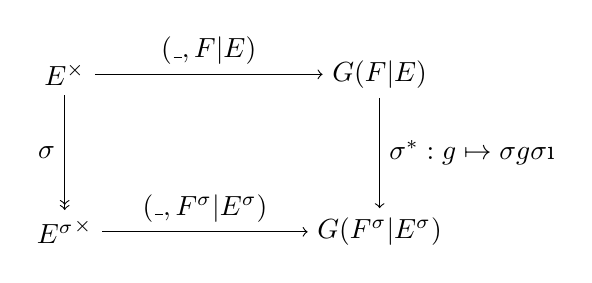
\begin{tikzpicture}[scale =1]
\node (D1) at (0,2)  {$E^\times$};
\node (D3) at (4,2)  {$G(F|E)$};
\node (D5) at (0,0)  {${E^\sigma}^\times$};
\node (D7) at (4,0)  {$G(F^\sigma|E^\sigma)$};

\draw[->] (D1) -> (D3) node[midway, above]{$(\_, F|E)$};
\draw[->] (D5) -> (D7) node[midway, above]{$(\_, F^\sigma | E^\sigma)$};
\draw[->] (D3) -> (D7) node[midway, right]{$\sigma^* : g \mapsto \sigma g \sigma\i$};
\draw[->>] (D1) -> (D5) node[midway, left]{$\sigma$};
\end{tikzpicture}
\end{center}

\item[($\Ac$2)] Sei $E'|E$ eine endliche Erweiterung und setze $F' = E'F$. Dann kommutiert
\begin{center}
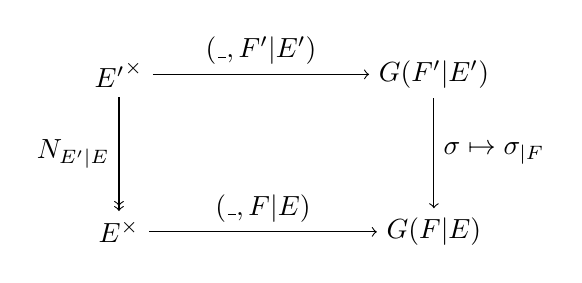
\begin{tikzpicture}[scale =1]
\node (D1) at (0,2)  {${E'}^\times$};
\node (D3) at (4,2)  {$G(F'|E')$};
\node (D5) at (0,0)  {${E}^\times$};
\node (D7) at (4,0)  {$G(F|E)$};

\draw[->] (D1) -> (D3) node[midway, above]{$(\_, F'|E')$};
\draw[->] (D5) -> (D7) node[midway, above]{$(\_, F | E)$};
\draw[->] (D3) -> (D7) node[midway, right]{$\sigma \mapsto \sigma_{|F}$};
\draw[->>] (D1) -> (D5) node[midway, left]{$N_{E'|E}$};
\end{tikzpicture}
\end{center}

\item[($\Ac$3)] Liegen endliche Körpererweiterungen $F|E'|E$ vor, sodass $F$ und $E'$ galoissch über $E$ sind, so kommutiert
\begin{center}
\begin{tikzpicture}[scale =1]
\node (D1) at (0,2)  {${E'}^\times$};
\node (D3) at (4,2)  {$G(F|E')$};
\node (D5) at (0,0)  {${E}^\times$};
\node (D7) at (4,0)  {$G(F|E)$};

\draw[->] (D1) -> (D3) node[midway, above]{$(\_, F|E')$};
\draw[->] (D5) -> (D7) node[midway, above]{$(\_, F | E)$};
\draw[->] (D7) -> (D3) node[midway, right]{$Ver$};
\draw[right hook->] (D5) -> (D1) node[midway, left]{};
\end{tikzpicture}
\end{center}
\end{itemize}
\item Die Zuordnung
\[ F \longmapsto \Nc_F := N_{F|E}F^\times \]
stiftet eine Eins-zu-Eins-Korrespondenz zwischen endlichen Erweiterung $F|E$ und offenen Untergruppen von endlichem Index von $E^\times$.\\
Insbesondere gelten hier dieselben Zusammenhänge bzgl. $\subseteq, \supseteq, \cap, \cdot$ wie in der globalen Version.
\end{itemize}
\Bem{Universelle Lokale Artin-Abbildung}
Sei $E|\Q_p$ endlich. Durch die Funktorialität der lokalen Artin-Abbildung erhalten wir folgenden stetigen Homomorphismus
\[ \phi : E^\times \Pfeil{} G(E^{ab}|E) \]
$\phi$ ist injektiv, aber nicht surjektiv. Dafür hat $\phi$ dichtes Bild und induziert folgenden Isomorphismus
\[ \widehat{\phi}:\widehat{E^\times} \Pfeil{\isom{}} G(E^{ab}|E) \]
wobei $\widehat{E^\times}$ die proendliche Komplettierung von $E^\times$ bezeichnet. Es gilt
\[ \widehat{E^\times} = \lim\limits_{D\leq_o E^\times \text{v.endl.I.}}E^\times / D =\lim\limits_{n} \Z/n\Z \times \O^\times_{E}/U^{(n)}_E = \widehat{\Z} \times \O_E^\times \]
da $\pi^{n\Z} \times U^{(n)}$ ein kofinales Teilsystem der offenen Untergruppen von endlichem Index von $E^\times$ bildet.

\Satz{}
Sei $F|E$ eine endliche, abelsche Erweiterung, wobei $E|\Q_p$ endlich sei. Dann bildet die lokale Artin-Abbildung die $n$-te \df{lokale Einseinheitengruppe}
\[ U_E^{(n)} := \left\lbrace
\begin{aligned}
E^\times && n = -1\\
\O_E^\times && n= 0\\
1 + \mf_E^n && n\geq 1
\end{aligned}
\right. \]
auf die $n$-te \df{Verzweigungsgruppe}
\[ G^n(F|E) := \set{\sigma \in G(F|E)}{ \sigma(x) \equiv x \mod{} \mf_E^{n+1} }\]
ab.

\Kor{Lokale Version des Satzes von Kronecker und Weber}
Ist $L|\Q_p$ abelsch und endlich, so liegt $L$ in einem Kreisteilungskörper über $\Q_p$.

\Def{Der Hilbertsche Klassenkörper}
Sei $K$ ein Zahlkörper. Definiere den \df{Hilbertschen Klassenkörper} $H(K)$ von $K$ durch den Klassenkörper zu $K^\times \A_{K,S_\infty}^\times$.\\
$H(K)$ ist dann die maximale, abelsche und überall unverzweigte Erweiterung von $K$. Es gilt
\[ G(H(K)|K) = \A_K^\times / K^\times \A_{K,S_\infty}^\times = \I / \P = Cl(K) \]

\Def{Strahlklassenkörper}
Sei $K$ ein Zahlkörper und $0\neq \af \subset \O_K$ ein Ideal.\\
Definiere die \df{Kongruenzuntergruppe mod ${\af}$} durch
\[C_K(\af) := \U(\af) K^\times / K^\times \subset C_K \]
wobei
\[ \U(\af) = \prod_{v} U_v(\af) \text{ wobei } U_v(\af) = \left\lbrace
\begin{aligned}
1 + \af \O_{K_v} && v\in S_f\\
K^\times_v = \C^\times && v \text{ komplex}\\
\{\text{ positive Elemente in }K^\times_v\} = \R_{> 0} && v \text{ reell}
\end{aligned}
\right. \]
Definiere den \df{Strahlklassenkörper mod ${\af}$} $K(\af)$ durch den Klassenkörper zu $C_K(\af)$.\\
Es gilt
\[ G(K(\af) / K) \isom{} C_K/C_K(\af) \isom{} Cl(K,\af)  \]
Ferner ist der Strahlklassenkörper mod $\af$ genau die endliche Körpererweiterung von $K$, die folgende Eigenschaften für jedes Primideal $\pf \subset \O_K$ erfüllt.
\begin{itemize}
\item $\pf\nmid \af$ $\Impl{}$ $\pf$ ist unverzweigt in $K(\af)$.
\item $\pf$ zerlegt sich voll in $K(\af)$ $\Gdw{}$ es existiert ein total positives $\alpha \in 1 + \af$ mit $\pf = (\alpha)$.
\end{itemize}

\Satz{}
Die offenen Untergruppen von endlichem Index von $C_K$ sind genau diejenigen Untergruppen, die eine Kongruenzuntergruppe umfassen.\\
Insbesondere ist jede endliche, abelsche Erweiterung von $K$ in einem Strahlklassenkörper enthalten.